\documentclass[11pt]{article}
\usepackage{graphicx} % Required for inserting images
\usepackage[top=2.5cm, bottom=2.5cm, left=2cm, right=2cm]{geometry}
\usepackage[T1]{fontenc}
\usepackage{wrapfig}
\usepackage{hyperref}
\usepackage[utf8]{inputenc}
\usepackage{multirow}
\usepackage{subcaption}
\usepackage{booktabs}
\usepackage{bookmark}
\usepackage{graphicx}
\usepackage{setspace}
\usepackage{listings}
\usepackage{xcolor}  % Opcional, per colors
\lstset{
  language=Python,
  basicstyle=\ttfamily\small,
  keywordstyle=\color{blue},
  commentstyle=\color{gray},
  stringstyle=\color{green!50!black},
  showstringspaces=false,
  numbers=left,
  numberstyle=\tiny\color{gray},
  frame=single,
  breaklines=true,
  captionpos=b,
  tabsize=4
}

\setlength{\parindent}{0in}
\usepackage{physics}
\usepackage{tikz}
\usepackage{tikz-3dplot}
\usepackage[outline]{contour} % glow around text
\usepackage{xcolor}
\usepackage{float}
\usepackage{makeidx}
\usepackage{fancyhdr}
\usepackage{pgfplots}
\usepackage{amsmath}
\pgfplotsset{compat=1.18}
\usepackage{caption}
\usepackage[english,catalan]{babel}
\setlength{\parskip}{11pt}
\usepackage{xcolor}
\usepackage{listings}
\usepackage{marginnote}
\usepackage{siunitx}
\usepackage{framed}
\usepackage{ulem}

\usepackage{titlesec}
\titleformat{\section}
  {\normalfont\Large\bfseries}
  {}
  {0pt}                
  {}  

\numberwithin{equation}{section}
\numberwithin{figure}{section}
\numberwithin{table}{section}

\begin{document}

\begin{titlepage}
    \centering
    \vspace*{\fill}

    {\Huge \bfseries Informes de Laboratori d'electromagnetisme\par}
    \vspace{2cm}
    
    {\Large \textbf{Grup A6}\par}
    \vspace{1cm}
    
    {\Large
    \begin{tabular}{c}
        NOM COGNOMS NIU \\
        NOM COGNOMS NIU \\
        NOM COGNOMS NIU \\
        NOM COGNOMS NIU \\
    \end{tabular}
    }
    
    \vspace{1cm}

    {\large Maig de 2025\par}

    \vspace*{\fill}
\end{titlepage}

\tableofcontents
\newpage
\vspace{10em}

\section{\huge \textbf{Pràctica 2}}

{}  % Títol petit en negreta

\vspace{0.5em}  % Espai vertical

{\Huge \textbf{Força entre corrents}}  % Títol gran

\vspace{1em}  % Espai abans del contingut

\begin{abstract}
    En aquesta pràctica estudiem la força magnètica entre dos fils amb corrent elèctric de mateixa intensitat, en concret, analitzem la seva relacció amb la magnitud d'intensitat dels fils i la dependència amb la distància que els separa. També s'aprofita el muntatge experimental per mesurar la component horizonal del camp magnètic terrestre. Les dades experimentals es tracten mitjançant el mètode dels mínims quadrats per obtenir paràmetres que es poden comparar amb valors teòrics. Aquests presenten diferències prou significatives respecte els nostres resultats tot i trobear-se dins l'interval d'incertesa, el que creiem que és degut a la gran complexitat del mètode experimental emprat.
\end{abstract}

\subsection{Introducció}\label{sec: PR2_intro}

En aquesta pràctica tenim per objectiu estudiar la força magnètica que es genera entre dos fils pels quals es fa passar corrent elèctric. També, aprofitarem el muntatge experimental per a mesurar la component normal del camp magnètic terrestre.

La força magnètica entre dos fils finits de corrent es calcula a través de la llei de Biot-Savart. Però tenint que la separació entre els fils de corrent és molt menor a la longitud d'aquests, podem arribar a considerar que el camp magnètic que rep un dels fils és el generat per un altre fil infinit situat a una distància d'ell. 

Aquesta aproximació ens facilita molt més els càlculs ja que podem trobar el camp magnètic generat per un fil infinit amb la llei d'Ampère, que ens dona com a resultat la següent expressió:

\begin{equation}\label{eq_PR2: PR2_camp_fil_infinit}
    B = \frac{\mu_0I}{2\pi r}
\end{equation}

I que la força mangètica que rep el fil d'una longitud $L$ és

\begin{equation}\label{eq: PR2_Fmagn_en_funcio_B}
    \vec{F} = I\oint d\vec{l}\times\vec{B}(\vec{r})
\end{equation}

Ens resultat que la força magnètica (el mòdul) té l'expressió següent:

\begin{equation}\label{eq: PR2_Fm_entre_fils}
    F = \frac{\mu_0I^2L}{2\pi r}
\end{equation}

Per mesurar la força magnètica entre dos fils de corrent i la seva dependència amb la intensitat de corrent que hi circula i amb la distància de separació entre ells utilitzarem una balança. Aquesta permet saber quan el sistema està en equlibri, és a dir, quan la força magnètica generada pels fils és compensada per una altra força d'igual direcció però sentit contrari. 

Aquesta altra força, que ha de ser fàcilment parametritzable, pot correspondre a la força gravetat  associada al fil superior. La qual mesurarem a través de les masses conegudes que col·locarem sobre la cassoleta que té aquest fil.

També pot correspondre a la força de torsió del sistema que conté el fil superior. La qual es pot mesurar a través de l'angle de gir resultant del fil superior al rebre la força magnètica.
 
La força gravetat segueix la següent equació

\begin{equation}\label{eq: PR2_Fgrav}
    F_{grav} = mg
\end{equation}

I la força de torsió

\begin{equation}\label{PR2_Ftorsio}
    F_{tor} = k\theta
\end{equation}

\subsection{Mètode Experimental}\label{sec: PR2_met_exp}

La balança de corrent està formada per un marc rectangular per on hi circula un corrent, gr. Aquest es troba sustentat pel fil de torsió i es troba sotmès a un equilibri entre la força del contrapes i la força entre fils. 

Per tal d'afavorir el moviment del rectangle conductor, les
connexions entre el marc i la font de corrent es fan usant gal·li fos. Els motius pels quals s'usa el gal·li són la seva baixa temperatura de fusió (29;76ºC) i al seu preu econòmic. El metall fos permet la mobilitat del marc i proporciona una connexió continua i gairebé sense presentar fricció. S'obren els pots de gal·li i es connecta el transformador de corrent de 9 V per fondre'l. 

A continuació, es posen en contacte
els pots de gal·li amb el marc rectangular, que té unes petites puntes sobresortint que entre perfectament en l'obertura de cada pot de gal·li. També es connecta el transformador amb el fil inferior, per a que aquest també tingui corrent circulant-hi.

%DIBUIX MUNTATGE

\begin{figure}[H]
    \centering
    \begin{subfigure}{0.4\textwidth}
        \centering
        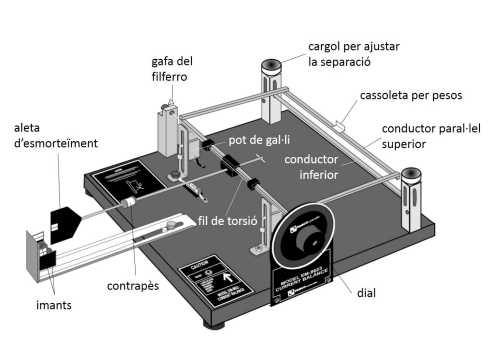
\includegraphics[width=0.5\textwidth]{PR2_dib_muntatge_parts.jpg}
        \caption{Parts de la balança usada en l'experiment.}
        \label{fig: PR2_dib_muntatge_parts}
    \end{subfigure}
    \hspace{0.1\textwidth}
    \begin{subfigure}{0.4\textwidth}
        \centering
        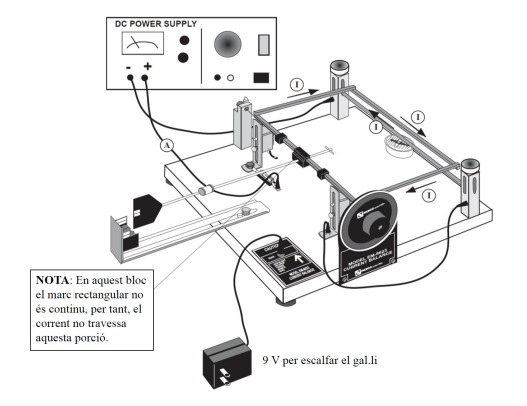
\includegraphics[width=0.5\textwidth]{PR2_dib_muntatge_corrent.jpg}
        \caption{Connexions per a fer circular corrent pels fils de la balança.}
        \label{fig: PR2_dib_muntatge_corrent}
    \end{subfigure}
\caption{Muntatge de la balança usada}
\end{figure}

La importància de la presa de mesures en aquesta pràctica recau en la calibració de la balança. Primerament, es col·loca la balana de tal forma que els cables siguin paral·lels al camp magnètic terrestre, seguint la direcció que ens indica la brúixola. Així, es pot eliminar la contribució del camp
magnètic terrestre, que alteraria els resultats. 

En segon lloc ajustem les potes de les potes de tal manera que la bombolla quedi al centre de l'espai disponible que te per moure's, fet que indica que està completament paral·lela al pla z. A continuació, ens assegurem que el dial de torsió del marc rectangular està al zero. 

Finalment, es mou el contrapès fins que la balança estigui estable i després es mou el cursor de marques, que conté uns imants per disminuir l'oscil·lació de l'aleta d'amortiment fins que ens quedin alineades amb la marca de l'aleta.

Després de fer una mesura, la balança pot quedar descalibrada (l'aleta d'amortiment no queda alineada amb el cursor de marques). Si aquest és el cas, cal tornar a calibrar la balança de nou.

Un cop la balança calibrada, la pràctica es divideix en 3 parts. En la primera part, es fan girar els cargols 5 voltes completes de tal forma que se separen els cables 5 mm més. A continuació es posa la massa de 5 mg i es connecta la font de corrent continu augmentant la intensitat ens que
s'equilibra la balança. Es repetirà el mateix procés per a les diferents masses, augmentant-les de 5 mg en 5 mg.

En la segona part de la pràctica, es posa la massa de 5mg sobre la cassoleta i es gira el dial ens que la balança torni a l'equilibri. Seguidament es repeteix el procés per les masses de 10, 15, 20 i 25 mg i a continuació es van separant els fils a I constant (girant les rodetes que desplacen el fil inferior) per a trobar el valor de $\mu_o$.

Finalment, en la tercera part de la pràctica es rota el sistema 90 graus per així detectar la component normal del camp magnètic terrestre. A continuació, es desconnecta la intesitat del cable inferior i pel superior es fa circular la major intensitat possible. Finalment, es gira el dial fins a equilibrar la balança.

%EQUILIBRAT DE LA BALANÇA

Per saber si el sistema es troba en equilibri cal fixar-nos en que les 3 línies, les dues del cursor de marques i la de l'aleta d'amortiment es trobin perfectament alineades. 

\iffalse
DIBUIX LLENGUETES
\begin{figure}[H]
    \centering
    \includegraphics[width=0.5\textwidth]{PR2_dib_llenguetes.jpg}
    \caption{Posició de les llenguetes quan balança està en equilibri.}
    \label{fig: PR2_dib_llenguetes}
\end{figure}
\fi

A la pràctica, l'aleta d'amortiment mai es quedava en una posició sense moviment. Així doncs, preniem com sistema en equilibri vàlid per a la mesura quan l'aleta patia la mínima osicil·lació possible, d'amplitud constant (igual desplaçament amunt i avall).

\subsection{Presentació i discussió de resultats}\label{sec: PR2_resultats}

\subsubsection{Dependència de la força mangètica amb la intensitat de corrent}\label{sec: PR2_Fm_intensitat}

En la primera part de la pràctica volem estudiar la relació que hi ha entre la intensitat que circula per un fil i la força que aquest rep a causa d’un altre fil pel que hi circula la mateixa intensitat. 

S’ha mesurat la intensitat necessària per fer circular pel fil perquè la força magnètica i la força gravitatòria de la massa de la balança estiguin en equilibri. S’ha fet la mesura per a 5 masses diferents, començant per 5 mg, i augmentant-la de 5 en 5 mg a cada nova mesura. Per a cada massa s’han
realitzat 3 mesures de la intensitat i se n’ha fet el promig.

Per comprovar la dependència s’ha representat la força en funció del quadrat de la intensitat i s’ha fet una regressió lineal. Els
valors obtinguts es mostren gràficament a la Fig. \ref{fig: regr_mvsI2}:

\begin{figure}[H]
    \centering
    \includegraphics[width=0.5\textwidth]PR2_regr_I2vsF.png}
    \caption{El quadrat de la intensitat en funció de la Força.}
    \label{fig: PR2_regr_I2vsF}
\end{figure}

La regressió té un coeficient de correlació de $R^2 = 0,98$. Axií doncs, que la força que un fil que transporta una intensitat I rep a causa d’un altre fil que transporta la mateixa intensitat I compleix la lineal proporcional: $F \sim I^2$.

El pendent de la recta de regressió ens permet trobar un valor aproximat de $\mu_0$. A partir de l’Eq. \eqref{eq: PR2_Fm_entre_fils} es dedueix que el pendent m serà $m = \frac{2\pi d}{\mu_0 L}$. Aïllant $\mu_0$ s’obté $\mu_0 = (0,413 \pm 0,091) · 10^{-6}\, T · m/A$, que difereix bastant (tot i tenir el mateix ordre de magnitud) del valor real que hem pres, de $4\pi · 10^{−7}\, T · m/A \,=\, 1,26 · 10^{−6}\, T·m/A$. 

Podem veure que el valor teòric no es troba dins l’interval d’incerteses considerat pel valor experimental i per tant els resultats no són compatibles. La incertesa instrumental associada a les mesures com per exemple la diferència de massa real respecte el marcat en les etiquetes i el que s'ha utilitzat per fer les regressions fa augmentar la discrepància entre els resultats. 

\subsubsection{Dependència de la força mangètica amb la distància de separació entre fils}\label{sec: PR2_Fm_sep}

En aquest segon apartat analitzarem com depèn la força magnètica amb la distància de separació entre fils per on circula corrent. 

Ho farem aconseguint mantenir en equilibri la força magnètica amb la força de torsió. Així doncs, primer cal obtenir la constant de torsió del fil. Es fixa una intensitat de (5,00 ± 0,01)A i es representen les dades de la força en funció de l’angle. Posteriorment es realitza una recta de regressió que ens permet trobar el valor de la constant k.

\begin{figure}[H]
    \centering
    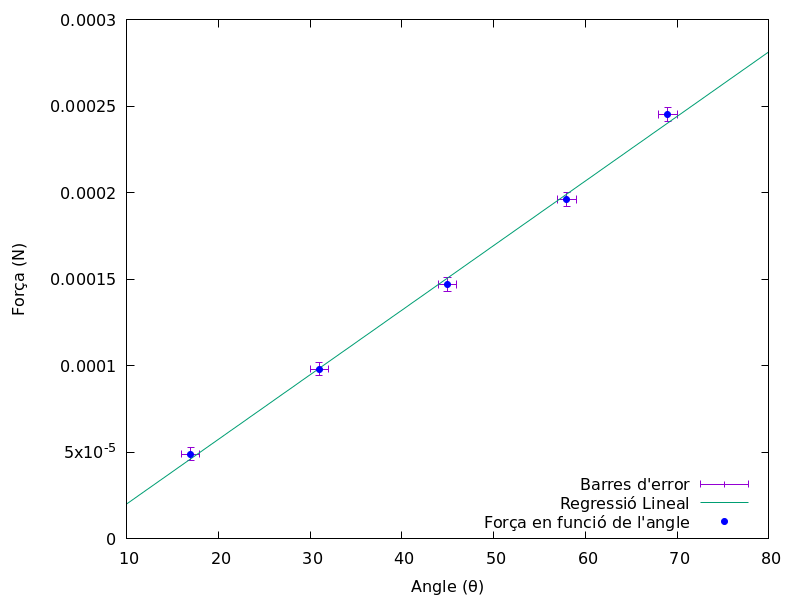
\includegraphics[width=0.5\textwidth]{PR2_regr_Fvstheta.png}
    \caption{Força en funció de l'angle de torsió.}
    \label{fig: PR2_regr_Fvstheta}
\end{figure}

La força que s’obté de la regressió és:

\begin{equation}\label{F_ktheta}
    F(\theta) = (3,73 \pm 0,10) \cdot 10^{-6}\, \theta
\end{equation}

Cal remarcar que la regressió lineal posseeix una ordenada a l’origen llunyana al zero ($(-1,75 \pm 0,50)·10^{-5}$). Tot i que aquesta ordenada d’origen no és menyspreable enfront els valors de la força,\textbf{ els resultats experimentals avalen que es pot no tenir en compte}. Aquesta ordenada d'origen pot haver aparegut a causa d’una imprecisa cal·libració de la balança, ja que es feia a ull. A més a més, el fet que la constant sigui positiva és un bon indicatiu, perquè la força ha d’augmentar linealment amb l’angle de torsió.

A continuació, mantenint fixa la intensitat anterior, es va variant la distància entre ambdós fils de corrent per calcular el valor de la permeabilitat magnètica $\mu_0$. 

Es representen els resultats obtinguts en la Fig. \ref{fig: PR2_regr_thetavsr} on es grafica la força respecte 1/r:

\begin{figure}[H]
    \centering
    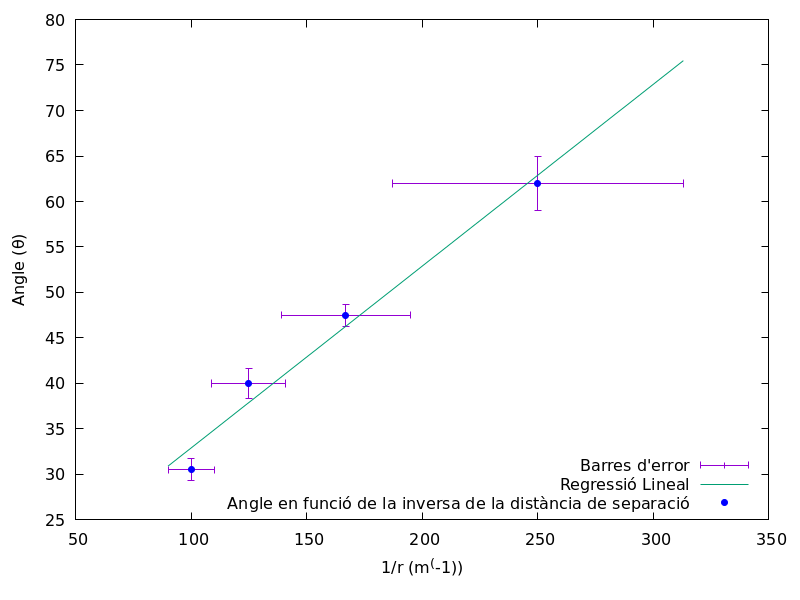
\includegraphics[width=0.5\textwidth]{PR2_regr_thetavsr.png}
    \caption{Força en funció de l’invers de la distància de separació entre fils de corrent.}
    \label{fig: PR2_regr_thetavsr}
\end{figure}

La regressió té un coeficient de correlació de $R^2 = 0,976$.
Aplicant la relació \eqref{F_ktheta} a l'equació que acabem de trobar i operant, s’obté que el valor de $\mu_o$ ve donat per l’equació $\mu_0 = \frac{2πm}{LI^2}$ on $m$ correspon al pendent de la regressió lineal. 

Aplicant el valor experimental s’obté que: $\mu_0 = (0,525 \pm 0,058) \cdot 10^{-6}\, N/A^2$. Tot i que el resultat tampoc és compatible amb l’esperat, sí és molt similar al resultat experimental de l’apartat anterior (tenint en compte els seus intervals d'incertesa, sí són compatibles) . 

De nou, cal considerar que la discrepància és deguda la complexitat en la mesura de les dades. Un error tan gran pot ser degut a factors que han influït en la mesura i que no s’han pogut tenir en compte en el càlcul de la incertesa, com ara petites vibracions de la taula o una calibració imprecisa de la balança. De fet, tenir aquesta mateixa discrepància en els dos càlculs de la permeabilitat magnètica al buit pot ser un indicatiu que la balança no estava ben calibrada, per això les dependències entre magnituds són correctes però els valors calulcats no. Tanmateix, el resultat és força proper al valor real.

Per millorar l'experiment i que els resultats numèrics fóssin més propers al teòric caldria considerar que la posició d'equilibri es devia trobar desplaçada del zero. També es podria recalibrar la balança de nou per no seguir arrossegant aquest error. Això és el que vam realitzar abans de començar la mesura del camp magnètic terrestre en la secció que ve a continuació.

\subsubsection{Camp magnètic terrestre}\label{sec: PR2_Bterra}

En aquesta última part de la pràctica es pretén mesurar la component horitzontal del camp magnètic terrestre. Per fer-ho, s’ha girat el dispositiu 90º de manera que sigui el camp de la Terra qui faci la força sobre el fil de corrent (recordem que fins ara el teníem paral·lel al camp de
la Terra perquè aquest no fes cap força sobre el fil). D’aquesta manera, mesurant la força que rep el fil es podrà trobar de quina magnitud és el camp causant d’aquesta força.

Per a una intensitat determinada, la força que rep el fil ve donada per l’equaci´o (2.2), i simmplement a¨ıllant el camp es podria trobar el seu valor. 

Fixant la intensitat a $(8,00 \pm 0,01)\,A$, trobem el valor de l'angle que permet tornar a deixar a equilibrar la balança, és a dir, igualem la força que rep el fil degut al camp magnètic amb la de torsió. La torsió obtinguda experimentalment és de $(19,5 \pm 2,3)$. 

Aprofitant el resultat de la constant de torsió trobada en la Sec. \ref{sec: PR2_Fm_sep}, podem trobar que la força magnètica que s’ha obtingut és de $F = (7,28 \pm 0,90) · 10^{-5}\,N$. 

De l’Eq \eqref{eq: PR2_Fmagn_en_funcio_B}, podem aïllar $B$ i obtenir que la component horitzontal del camp magnètic de la Terra al laboratori de la Universitat Autònoma, és $B = (3,08 \pm 0,59)·10^{-5}\,T$. El valor real que hem agafat és de $B = 2,53·10^{−5}\,T$ \footnote{Valor obtingut d'un document de la R.S.E.F. on s'havia mesurat la component horitzontal del camp magnètic a Salamanca}. Per tant, com el valor experimental es troba dins l’interval d’incerteses, és compatible amb el resultat esperat.

Només hem pogut estudiar la component horitzontal del camp magnètic terrestre perquè la component vertical d’aquest és perpendicular al conductor i per tant la balança que tenim no permet fer la seva mesura.

També podem observar que el fet d'haver desplaçat la balança, ens ha obligat a recalibrar aquesta de nou. Això pot haver influit en què els resultats de c'alcul del camp magnètic sí continguin el valor teòric en el seu interval d'incerteses.

\subsection{Conclusions}\label{sec: PR2_concl}

En vista dels resultats es comprova que la dependència en $I^2$ i en $1/r$ de la força magnètica, efectivament és lineal, tal com predien les equacions trobades per un sistema de fils parl·lels pels quals circula una mateixa intensitat. 

També s’ha obtingut experimentalment el valor de $\mu_0$ de dues maneres diferents, obtenint en ambdós casos valors que discrepen amb al valor teòric acceptat però similars entre ells.

Concluim doncs, que el mètode experimental és prou bo tot i els errors que té associats. No obstant, veiem que el calibratge inicial de balança és molt determinant en els resultats numèrics, en el nostre cas, s'hauria de tenir en compte que el punt d'equilibri de la balança es trobava fora del zero o es podria haver recalibrat la balança de nou abans de començar a fer les mesures de cada part de l'experiment.

La component horitzontal del camp magnètic terrestre a la Universitat Autònoma és de $B_{T_{norm}}= (3,08 \pm 0,59)\cdot10^{-5} \, T$ que conté dins del seu rang d’incertesa el valor teòric mesurat a Salamanca (el qual utilitzem de referència).

\newpage

{\huge \textbf{Pràctica 6}}  % Títol petit en negreta

\vspace{0.5em}  % Espai vertical

{\Huge \textbf{Feixos de raigs catòdics}}  % Títol gran

\begin{abstract}
     En aquesta pràctica s'estudia el comportament d'un feix de raigs catòdics sota un camp elèctirc i un camp magnètic amb l'objectiu de determinar les propietats de les partícules que els conformen. Concretament, analitzant les desviacions del feix dels raigs sota aquests camps s'obté la relació entre la càrrega i la massa de les partícules que ens permet determinar que són electrons.
\end{abstract}

\subsection{Introducció Teòrica}
En aquesta pràctica estudiarem com es desvia el feix de raigs catòdics sota el camp elèctric generat per un condensador i el camp magnètic generat per unes bobines de Helmoholtz. A través de les equacions d'aquests, podrem determinar propietats de les partícules que conformen els raigs. Concretament, els objectius que ens plantegem són:

\begin{list}{$\ast$}{\leftmargin=1em}
    \item Caracteritzar el camp elèctric generat pel condensador no ideal que usem a l'experiment a través d'un factor experimental.
    \item Determinar i explicar el comportament dels raigs catòdics sota el camp elèctric i el camp magnètic. Estudiar-ho per diferents intencitats i potencials aplicats als generadors de camp.
    \item Determinar, amb dos mètodes diferents, de què estan fets els raigs catòdics trobant la relació entre la càrrega i la massa de les seves partícules.
\end{list}


%DESV E
Primerament, estudiarem la desviació del feix degut a un camp elèctric perpendicular a la velocitat; aplicant una diferència de potencial $V_p$ entre dues plaques plano-paral·leles. Degut a què la distància entre plaques $d$ (= 54 mm) és de l'ordre del tamany d'aquestes, no podem considerar el sistema com un condensador de plaques plano-paral·leles ideal amb un camp uniforme $E=V/d$. En comptes, seguirem considerant-lo uniforme però modificarem l'expressió mitjançant una constant $k$ que tindrà en compte els efectes de vorada i que trobarem experimentalment.
\begin{equation}
    E = \frac{kV_p}{d}
    \label{eq: Camp E}
\end{equation}

Si les partícules de les quals està format els raigs catòdics (de massa $m$) tenen càrrega elèctrica $q$, aquestes es desviaran cap a un dels dos elèctrodes; al càtode si són negatives i a l'ànode si són positives. I la trajectòria que seguiran serà una paràbola parametritzada per l'Eq. (\ref{eq: trajectoria}), ja que el camp és uniforme i en direcció $y$.
\begin{align}    \label{eq: trajectoria}
    &x = v_0 t      &y = -\frac{qEt^2}{2m}
\end{align}

On $v_0$ és la velocitat en direcció $x$ que tenen inicialment les partícules al sortir del filament.
Donat que un cop emeses les partícules, aquestes es veuen accelerades degut al voltatge aplicat $V_a$; per conservació de l'energia, la velocitat ha de ser:
\begin{equation}
    \frac{1}{2}mv_0^2=qV_a
    \label{eq: Energia}
\end{equation}

Tot i això, no es pot veure el moviment d'una partícula individual en funció del temps, sinó que es veu una corba formada per moltes partícules en diferents moments de la trajectòria. L'expressió d'aquesta corba com una funció de $x$ ($y$ = $f(x)$)  s'obtè combinant les Eqs. (\ref{eq: Camp E}), (\ref{eq: trajectoria}) i (\ref{eq: Energia}):
\begin{equation}
    y = \frac{kV_px^2}{4dV_a}
    \label{eq: parabola}
\end{equation}

Per últim, queda determinar experimentalment la constant $k$ a partir del pendent $m$ de la recta de regressió lineal de $y$ en funció de $x^2$ i de l'equació (\ref{eq: parabola}):
 \begin{equation}
      k =\frac{4mdV_a}{V_p}
      \label{eq: k}
 \end{equation}

%DESV M
\vspace{1cm}

Per calcular el radi de corvatura i posteriorment la relació $\frac{q}{m}$ de les partícules dels raigs catòdics necessitem caracteritzar la trajectòria de les partícules carregades sota un camp magnètic uniforme. En l'experiment, el camp d'inducció magnètica està generat per unes bobines de Hemholtz que aproximadament produeixen el camp uniforme 
\begin{equation}
    \vec{B}=\frac{32\pi nI}{5\sqrt{5}r}\cross10^{-7} \quad \hat{z}\quad Wb/m^2.
    \label{eq: B}
\end{equation}
Per altra banda, la llei de Lorentz dicta que una partícula carregada negativament sota un camp d'inducció magnètica, $\vec{B}$, pateix una força
\begin{equation}
    \vec{F}=q\vec{v}\cross\vec{B}.
    \label{eq: Lorentz} 
\end{equation} 
En el nostre cas, $\vec{v}$ és perpendicular a $\vec{B }$ i, per tant, les partícules dels raigs catòdics seguiran una trajectòria circular d'equació
%Aquesta força, al ser sempre perpendicular a la velocitat i tenint en compte que en el nostre sistema la velocitat de les partícules carregades, $\vec{v}$, és perpendicular a $\vec{B }$ induirà un moviment circular a les partícules de radi R. La trajectòria de les partícules carregades del nostre sistema complirà
\begin{equation}
    R=\frac{x^2+y^2}{2y}.
    \label{eq: radi}
\end{equation}
On $R$ és el radi del cercle i hem agafag el centre de coordenades a l'inici del tub de raigs catòdics i l'eix $X$ del sistema paral·lel a la direcció de sortida dels raigs.

Ara, per calcular la relació entre la intensitat de corrent de les bobines de Helmoholtz i el radi de corvatura de les partícules cal igualar la força centrípeta a la força de Lorentz, i obtenim 
\begin{equation}
    Bqv=\frac{mv^2}{R}
    \label{eq: fc=fl}
\end{equation}
que combinada amb l'Eq. (\ref{eq: B}) ens dona la relació entre el radi i la intensitat de corrent
\begin{equation}
    R=K\frac{1}{I} \quad on \quad K=\frac{mv5\sqrt{5}r}{32\pi n}\cross 10^7.
    \label{eq: IvsR}
\end{equation}
Tenint en compte l'Eq. (\ref{eq: fc=fl}) i la llei de la conservació de l'energia mecànica, $qV_a = \frac{1}{2}mv^2$, s'obté 
\begin{equation}
    \frac{q}{m}=\frac{2V_a }{B^2R^2}
    \label{eq: q/m}
\end{equation}
que ens permetrà calcular la relació $\frac{q}{m}$ de les partícules.


\vspace{1cm}

Una altre manera de calcular la relació càrrega/massa de les partícules dels raigs catòdics és igualant forces elèctriques i magnètiques. Fent-ho, arribem a la següent equació:

\begin{equation}\label{eq: Fm=Fe}
    qE = qvB
\end{equation}

Amb la que es troba que la velocitat vindrà donada pel quocient:

\begin{equation}
    v = \frac{E}{B}
\end{equation}

Podem obtenir el radi de la trajectòria circular deguda només a la desviació magnètica com hem explicat prèviament.

De les Eqs \eqref{eq: Fm=Fe}, \eqref{eq: fc=fl} es pot deduir l'equació que emprem en la secció \ref{sec: desv_em} per a calcular la relació càrrega/massa a partir de les nostres dades experimentals:

\begin{equation}
    \frac{q}{m}=\frac{E}{RB^2}=\frac{kV_p}{dK^2I^2R}
\end{equation}

\newpage
\subsection{Mètode Experimental}

El procediment experimental seguit ha constat de diversos passos que estan explicades detalladament al guió de la pràctica. 
Primerament, s'ha aplicat una diferència de potencial al tub de raigs catòdics i s'ha fet visible el feix lluminós dels raigs. Tot seguit s'ha estudiat la desviació d'aquest feix al aplicar diferents valors de camp elèctric (generat per un condensador planoparal·lel) o magnètic (generat per unes bobines de Hemholt) ambdós uniformes i perpendiculars. Per poder determinar punts de la trajectòria del feix de raigs catòdics, hem fotografiat el raig usant un dispositiu mòbil i cobrint-nos amb un material opac per tal de tenir més contrast. Posteriorment, aquestes fotografies han estat processades digitalment.

En el cas del camp magnètic, per poder estudiar la relació entre el radi de corvatura del feix i la intensitat de corrent de les bobines de Helmholtz, s'ha fotografiat el raig per les següents intensitats:  $0.1A, 0.2A, 0.3A, 0.4A, 0.5A, 0.6A, 0.7A, 0.8A$. Igualment, per determinar la relació entre el radi de corbatura i el potencial aplicat hem usat els següents potencials: $2kV, 3kV, 4kV$ i $5kV$.

En aquest punt, mitjançant un dispositiu mòbil s'han fotografiat els diferents casos. Aleshores, s'ha processat cada imatge, ja a ordinador, amb un programa d'edició que permet ajustar les mesures del feix mitjançant els propis píxels de les fotografies comparats amb les marques de la regla. Es a dir, comptant aquests píxels i convertint-los a centímetres. Aquest doncs, ha estat el procediment seguit: triar a consciència diversos punts del feix i donar-ne la posició (x,y) més exacta possible, sempre sent possibles errors degut al processat de la fotografia o al desplaçament de píxels. Més precisament, s'ha aplicat una grid (cuadrícula) sobre els espais compresos entre cada marca de la regla, coincidint amb cada variació de 1 cm, per cada eix. Així, per cada una de les imatges s'ha establert una conversió píxel/cm. S'inclou un exemple gràfic (\ref{fig: ex_grid}) a continuació:

\begin{figure}[H]
    \centering
    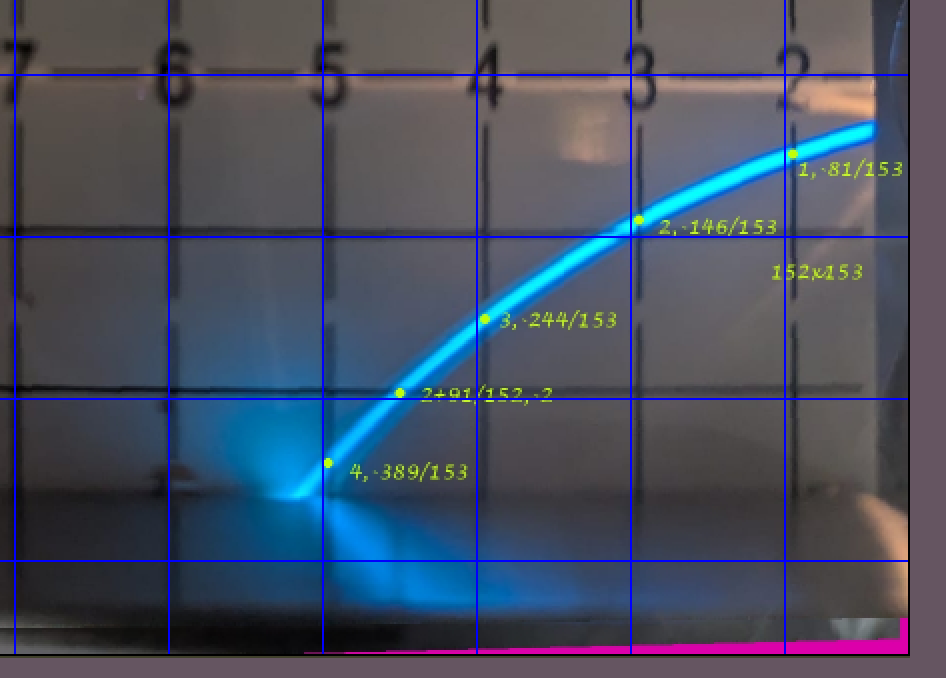
\includegraphics[scale=0.3]{Ex_grid.png}
    \caption{Imatge modificada després de l'aplicació de la grid corresponent amb la seva relació px/cm: 152/1 i 153/1.}
    \label{fig: ex_grid}
\end{figure}


Llavors, per cada un dels punts s'ha determinat la posició dins la grid comptant els píxels de separació amb la frontera del quadrat corresponent, i finalment, s'han convertit a centímetres. Amb aquests resultats, s'ha estudiat la desviació de la trajectòria; fet crucial pel desenvolupament de la prova, doncs les partícules del feix es poden identificar segons aquest comportament.

\newpage
\subsection{Resultats i discussió}

\subsubsection{Desviació electroestàtica}\label{sec: desv_electr}

En subministrar una diferència de potencial a les plaques s'observa com el raig es desvia cap al càtode\footnote{Les imatges de la desviació electroestàtica (Fig.(\ref{fig: Desv E})) es troben a l'annex (\ref{sec: imatges}) }. Per tant, les partícules de les què està compost els raigs catòdics tenen una càrrega negativa.

 Per comprovar que les trajectòries es tracten de paràboles hem fet una regressió de les $y$ en funció de les $x^2$, com es mostra a la figura (\ref{fig: Regressió Desv E}). Aquestes tenen els següents coeficients de correlació \footnote{Les regressions lineals en detall es troben a l'annex \ref{sec: Reg}}:
 r$^2$ = 0.9777, 0.9973, 0.9940, 0.9832. Confirmant que les partícules segueixen una trajectòria parabòlica.
\begin{figure}[h]
    \centering
    \begin{minipage}{0.75\textwidth}
    \centering
        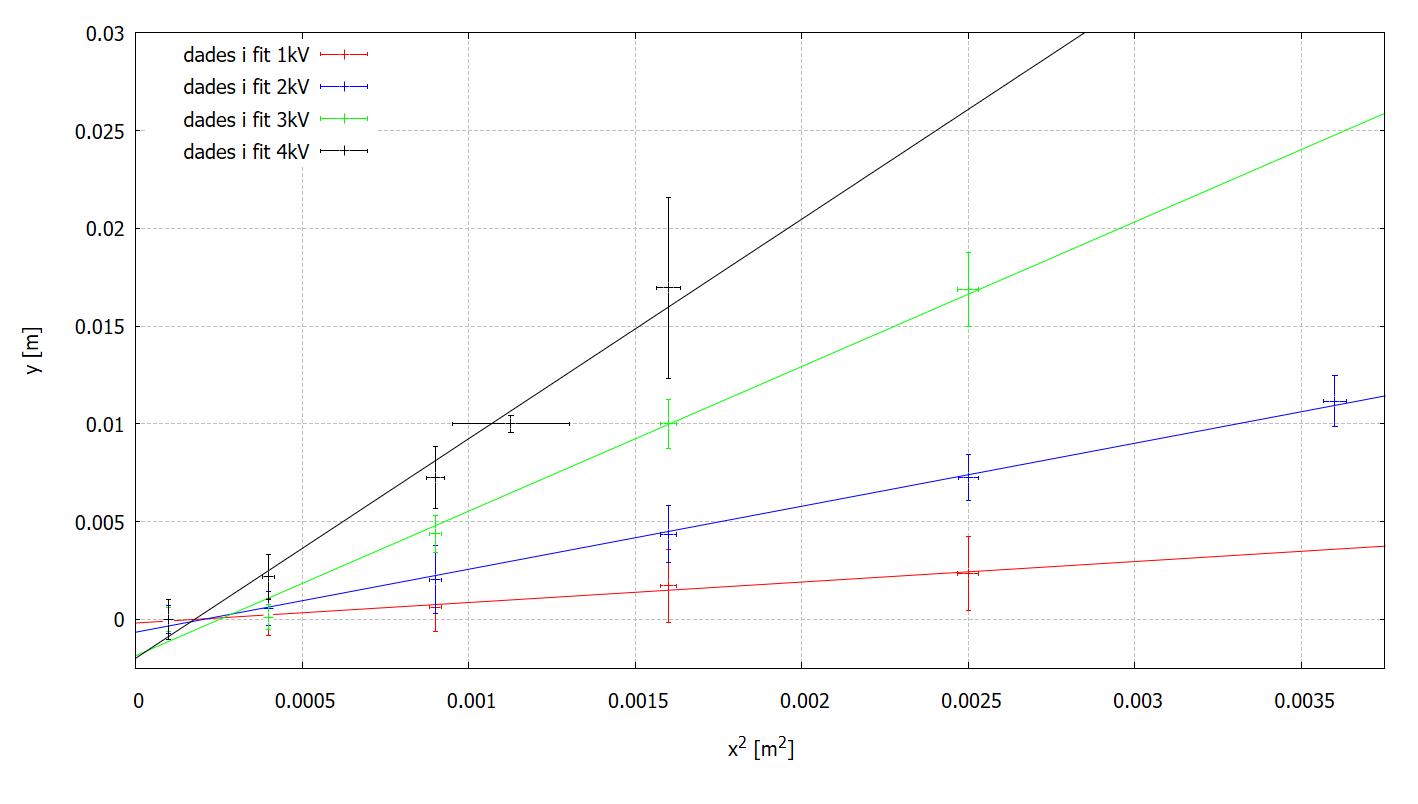
\includegraphics[width=1\linewidth]{Plot yvsx.PNG}
        \caption{Regressió de $y$ en funció de $x^2$  de la desviació deguda al camp elèctric}
        \label{fig: Regressió Desv E}
    \end{minipage}
\end{figure}

A la taula \ref{tab:kvsVp} podem observar els diferents valors que pren $k$ \footnote{El càlcul de les incerteses es mostra a l'anex \ref{sec: incerteses}} en funció del potencial entre plaques $V_p$, obtinguts a partir del pendent d'aquestes regressions lineals juntament amb l'Eq. (\ref{eq: k}). Observem que la $k$ no és constant i que augmenta amb la diferència de potencial. Fent una regressió lineal entre $V_p$ i $k$ obtenim que hi ha una relació lineal entre els dos amb un coeficient de correlació r$^2$ = 0.9737 i una equació de la recta: $k = 0.453 \cdot 10^{-3}\, V^{-1}  \cdot V_p + 0.45$.


\begin{figure}[h]
    \centering
    \begin{minipage}{0.45\textwidth} 
        \centering
        \begin{tabular}{|c|c|}
            \hline
            $V_p$ (V)	&	$k$	\\\hline
            (1000 ± 200)	&	(0.87 ± 0.64)   \\\hline
            (2000 ± 200)	&	(1.35 ± 0.22)	\\\hline
            (3000 ± 200)	&	(1.94 ± 0.25)	\\\hline
            (4000 ± 200)	&	(2.17 ± 0.26)	\\\hline           
        \end{tabular}
        \captionof{table}{Resultats experimentals de les constants $k$ del condensador per cada valor del potencial $V_p$.}
        \label{tab:kvsVp}
    \end{minipage}
\end{figure}


\subsubsection{Desviació magnetoestàtica}\label{sec: desv_magn}
Després de comprovar a la Secció \ref{sec: desv_electr} que les partícules dels ràigs catòdics tenen càrrega negativa, n'estudiarem la interecció amb el camp magnètic, substancialment uniforme, generat per unes bobines de Hemholtz. 
Al aplicar el camp, com era d'esperar, hem observat que els ràigs es corbaven i ens hem disposat a estudiar les dependències d'aquesta corba i el seu radi amb la intensitat del corrent de les bobines i amb el potencial dels raigs catòdics.

Per calcular el radi de la trajectòria de les partícules dels raigs catòdics en funció de la intensitat de corrent de les bobines hem usat l'Eq. (\ref{eq: radi}) que defineix el radi com el pendent de la recta de regressió entre $x^2+y^2$ i $2y$. A la Fig. (\ref{fig: regressio_1}) hem representat una selecció d'aquestes regressions i ja podem veure com a mesura que augmenta la intensitat, el pendent de la recta, és a dir el radi de les partícules, disminueix. 
\begin{figure}[H]
    \centering
    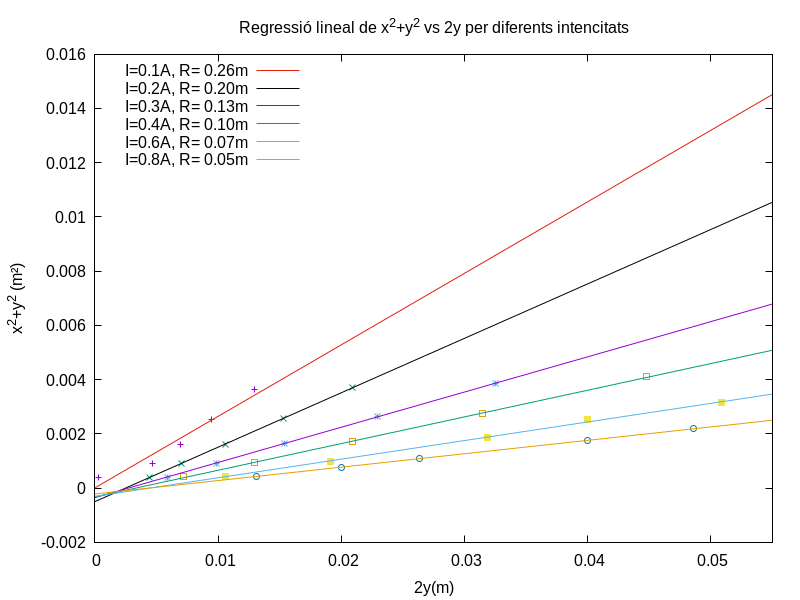
\includegraphics[scale=0.3]{regressio_1.png}
    \caption{Regressió per diverses intensitats de les bobines de Hemholtz de $x^2+y^2$ en front $2y$ on $y$ i $x$ són punts de la trajectòria dels raigs catòdics. La pendent de les rectes és el radi de corvatura de la trajectòria.}
    \label{fig: regressio_1}
\end{figure}
Aplicant diverses intensitats a les bobines de Helmholtz hem obtingut els radis de corvatura de la Taula \ref{tab:RvsI} que es pot trobar a l'annex conjuntament amb el càlcul d'incerteses. Amb aquestes dades (excloent l'última dada ja que té massa incertesa a causa de l'amplada del feix dels raigs) hem construit la gràfica de la Fig. (\ref{fig: RvsI}) on es mostra que la variació del radi corvatura és lineal amb la variació de la inversa de la intensitat. 
Al fer la regressió lineal del radi en funció de l'inversa de l'intensitat hem obtingut la recta
\begin{equation}
    y=x(0.03976\pm0.0006)+(0.0002\pm0.0016)
\end{equation}  
amb un coeficient de determinació de $r^2\approx0,99$. Per tant, la relació és certament lineal tot verificant la predicció de l'Eq.(\ref{eq: fc=fl}) ja que a més a més, l'ordenada a l'origen inclou el zero. El radi de corvatura és inversament proporcional a la intencitat a causa de què al augmentar la intensitat de les bobines de Hemholtz el camp d'inducció magnètica augmenta provocant que les partícules rebin més força centrípeta què alhora provoca que el radi de la trajectòria disminueixi.
\begin{figure}[h]
    \centering
    \begin{minipage}{0.45\textwidth}
        \centering
        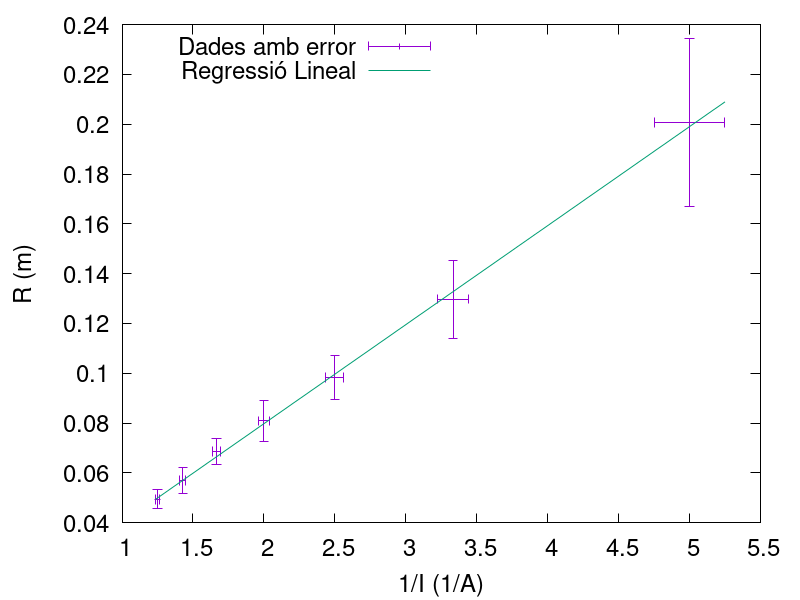
\includegraphics[width=\textwidth]{RvsI.png}
        \caption{Regressió de R en funció de $1/I$ excloent l'últim punt que perd la tendència.}
        \label{fig: RvsI}
    \end{minipage}
    \hfill
    \begin{minipage}{0.45\textwidth} 
        \centering
        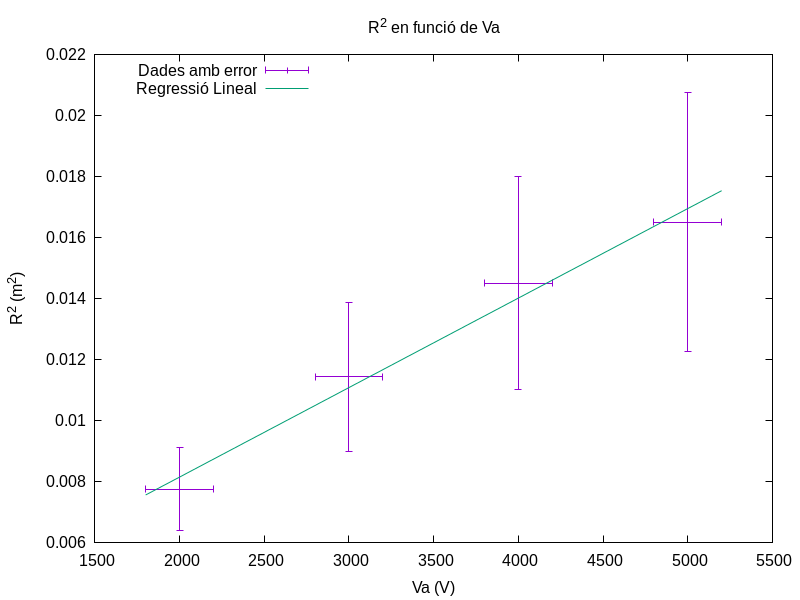
\includegraphics[width=\textwidth]{RvsVa.png}
        \caption{Regressió dels punts experimentals de $R^2$ en funció de $V_a$. Veiem que la relació és clarament lineal.}
        \label{fig: RvsVa}
    \end{minipage}
\end{figure}
Per calcular el radi de la trajectòria de les partícules dels raigs catòdics en funció del potencial d'acceleració d'aquestes usem l'Eq. (\ref{eq: radi}) que defineix el radi com el pendent de la recta de regressió entre $x^2+y^2$ i $2y$. Alicant diferents potencials a les bobines de Helmoholtz s'obtenen els radis de corvatura de la Taula \ref{tab:RvsVa} que es troba a l'annex. Amb aquestes dades hem construit la gràfica de la Fig. (\ref{fig: RvsVa}) on es mostra que la variació de $R$ és quadràtica amb la variació de $V_a$. Al fer la regressio lineal de $R^2$ respecte $V_a$ hem obtingut la recta
\begin{equation}
    y=x(2.93\times10^{-6}\pm0.27\times10^{-6})+(2.28\times 10^{-3}\pm9.8\times10^{-4})
\end{equation}  
amb un coeficient de determinació $r^2=0.98$. Per tant, la relació és certament lineal (quadràtica respecte $R$) i corrobora l'Eq. (\ref{eq: q/m}).


Finalment, amb l'Eq. (\ref{eq: q/m}) hem obtingut la relació $\frac{q}{m}$ de les partícules dels raigs catòdics
\[
\boxed{\frac{q}{m}=(-4.16\pm0.88)\cross10^{11}\quad \mathrm{\frac{C}{Kg}.}}
\]
Per fer-ho hem calculat la regressió lineal ajustada entre $2V_a$ i $B^2R^2$. Així, hem obtingut la recta $y=(4.16\pm0.38)x - (1412.64\pm791.71)$ amb un coeficient de determinació de $r^2\approx0.98$. El pendent d'aquesta recta ens ha donat el valor de $\frac{q}{m}$ i després hem afegit l'insertesa instrumental al resultat. La linealitat dels punts indica que els nostres resultats concorden amb la teoria ja que com veiem a l'Eq. (\ref{eq: q/m}) la relació ha de ser lineal. 
Per altra banda, el valor tabulat\footnote{Valor obingut de la pàgina del NIST: "The NIST Reference on Constants, Units and Uncertainty".} de la relació $\frac{q}{m}$ dels electrons és de $\frac{q}{m}=(-1.76\times10^{11}\pm5.5\times10^{2}) \frac{C}{Kg}$ que    com podem veure no és compatible amb el nostre resultat però sí que coincideix en ordre de magnitud. Això pot ser per diversoso motius com que, com es veu a la Secció \ref{sec: traj_no_rect} el camp magnètic generat per les bobines de Hemholtz no és del tot uniforme o que el feix dels raigs catòdics té un gruix considerable que fa molt difícil l'obtenció dels punts experimentals.


\subsubsection{Desviació electromagnètica}\label{sec: desv_em}

En aquest tercer apartat ens interessem la relació càrrega/massa de les partícules dels raigs catòdics per a comprovar que aquesta coincideix amb la de l'electró. 

Tenint en compte el que ja hem pogut observar en els apartats anteriors: la desviació parabòlica a l'aplicar un camp elèctric $\vec{E}$ i desviació circular a l'aplicar el camp d'inducció magnètica $\vec{B}$, el que ens interessa en aquest tercer apartat és aplicar els dos camps a la vegada de tal manera que de les dues deflexions estiguin al mateix pla però en amb direccions oposades de manera que aconseguim que la trajectòria dels raig catòdics no es vegi desviada.

Primerament, hem trobat el valor de la diferència de potencial aplicat entre les plaques amb el qual la desviació de la trajectòria rectilina paral·lela a l'eix de les abscisses és mínima. En concret hem hagut d'aplicar una diferència de potencial $Vp = (0,85 \pm 0,20 )\, kV$ per compensar un camp magnètic generat per bobines amb intensitat de $I = (0,10 \pm 0,01 )\, mA$ i un potencial $Va = 3\, kV$ per a l'accelaració de les partícules dels raigs catòdics.

Fixant aquests valors de pontencial i d'intensitat, posteriorment es suprimeix el camp elèctric $\vec{E}$ per poder mesurar el radi de la trajectòria que deguda només de la desviació magnètica d'igual manera que en la secció \ref{sec: desv_magn}.

Amb aquestes dades hem obtingut el radi de la trajectòria pel mètode dels mínims quadrats, on aquest venia donat pel pendent de la recta de regressió lineal.

Essent la recta en qüestió: 
\begin{equation}
    y=(0,244 \pm 0,033)x + (-2,0 \pm 1,3) \times10^{-4}
\end{equation}  
amb un coeficient de determinació $r^2=0.96$ i  donant un resultat de $R = (0.243 \pm 0.039) \, m$.

La constant del condensador $k$, amb valor $(1,06 \pm 0,28)\, V^{-1}$ la qual té en compte els efectes de vorada de les plaques, la hem obteningut com hem fet prèviament a la secció \ref{sec: desv_electr}. 

D'altra banda la constant de les bobines de Hemholtz $K$ ve determinada per la geometria d'aquestes, com s'explica en la secció \ref{sec: desv_magn}.

Per últim, un cop hem trobat la relació càrrega-massa $q/m$\footnote{El càlcul de les incerteses associades a aquest resultat es presenten en l'annex \ref{sec: incerteses}} podem comparar-la amb la relació e/m, on e correspon a la càrrega d'un electró i m a la seva massa.

\[
\boxed{\frac{q}{m}=(-3,8 \pm 1,7)\cdot 10^{11}\, C/Kg.}
\] 

Tot i que coincideix en ordre de magnitud, observem que el nostre resultat q/m queda lluny del resultat que esperàvem. De fet, el valor trobat no arribar a ser compatible amb l'esperat ja que no l'inclou en el seu rang d'incerteses. 

Cal notar que la trajectòria mesurada és perfectament rectilínia tot i haver-se considerat així per poder fer els càlculs. No queda com la trajectòria que podem observar quan no hi ha aplicat ni camp elèctric ni camp magnètic, la qual s'apropa molt més a la liniealitat constant al llarg del feix. 

Això és degut a la no uniformitat que s'ha suposat en el tractament matemàtic tant del camp elèctric com del camp magnètic. Per una banda el condensador no és ideal, ja que les plaques són petites, lluny de poder-se considerar infinites però és cert que aquests efectes de vorada ja els tenim en compte al calcular la seva $k$ mitjançant la regressió lineal. D'altra banda, el solenoide emprat no és ideal tampoc, ja que la seva longitud no és molt més gran que el radi. Això implica que el camp en l'interior sigui de magnitud més gran com més aprop de l'eix central de la bobina ens trobem. Aquest és l'efecte que podem observar en les imatges, podem veure com la trjaectòria dels raigs catòdics presenta més desviació deguda al camp magnètic quan passa pel centre del solenoide.

\subsection{Conclusions}
A partir de l'experimentació amb els raigs catòdics, s'han obtingut resultats que confirmen el comportament esperat dels electrons sota la influència de camps elèctrics i magnètics. 
    
En aplicar una diferència de potencial en les plaques del condensador, s'ha observat que el feix de partícules es desvia en la direcció contrària al camp elèctric. Al travessar una regió amb un camp magnètic uniforme, la trajectòria del feix canvia a una corba amb un radi que té dependència inversament proporcional amb el quocient càrrega/massa ($q/m$) i amb la intensitat del camp magnètic. 

Així doncs, s'ha verificat que els feixos tractats, els raigs catòdics, estan compostos per partícules carregades negativament i que efectivament, són electrons. Tanmateix, fixant-nos en les diferències numèriques trobades al comparar els nostres resultats amb els esperats podem concloure que el disseny experimental és prou bo per a estudiar la relació càrrega/massa de les partícules dels raigs catòdics però no suficientment exacte. 

\newpage

\appendix{Annex}
\section{Annex}

\subsection{Resultats experimentals}\label{taules_dades_exp}

\subsubsection{Resultats experimentals Pràctica 2}\label{PR2_taules_dades_exp}

%TAULES DADES EXPERIMENTALS

\begin{table}[h!]
\centering
\caption{Taula d'intensitats de corrent (A) en funció de la massa (mg)}
\begin{tabular}{|c|c|c|c|c|c|}
\hline
\textbf{Massa (mg)} & \textbf{5 $\pm$ 0.4 } & \textbf{10 $\pm$ 0.4 } & \textbf{15 $\pm$ 0.4} & \textbf{20 $\pm$ 0.4 } & \textbf{25 $\pm$ 0.4 } \\
\hline
 & 2.71 $\pm$ 0.01 & 4.38 $\pm$ 0.01 & 5.21 $\pm$ 0.01 & 6.23 $\pm$ 0.01 & 7.70 $\pm$ 0.01 \\
\textbf{I (A)} & 2.66 $\pm$ 0.01 & 4.2 $\pm$ 0.012 & 5.13 $\pm$ 0.01 & 6.44 $\pm$ 0.01 & 7.58 $\pm$ 0.01 \\
 & 2.71 $\pm$ 0.01 & 4.10 $\pm$ 0.01 & 5.47 $\pm$ 0.01 & 6.38 $\pm$ 0.01 & 7.81 $\pm$ 0.01 \\
\hline
\end{tabular}
\end{table}

\begin{table}[H]
\centering
\caption{Taula d'angles ($\theta$) en funció de la massa (mg)}
\begin{tabular}{|c|c|}
\hline
\textbf{Massa (mg)} & \textbf{Angle ($\theta$)} \\
\hline
5 $\pm$ 0.4   & 17 $\pm$ 1 \\
10 $\pm$ 0.4  & 31 $\pm$ 1 \\
15 $\pm$ 0.4  & 45 $\pm$ 1 \\
20 $\pm$ 0.4  & 58 $\pm$ 1 \\
25 $\pm$ 0.4  & 69 $\pm$ 1 \\
\hline
\end{tabular}
\end{table}

\begin{table}[H]
\centering
\caption{Taula d'angles ($\theta$) en funció de la distància de separació entre fils (mm)}
\begin{tabular}{|c|c|c|c|c|}
\hline
\textbf{Distància separació (mm)} & \textbf{4 $\pm$ 1} & \textbf{6 $\pm$ 1} & \textbf{8 $\pm$ 1} & \textbf{10 $\pm$ 1} \\
\hline
\textbf{Angle ($\theta$}) & 64 $\pm$ 1  & 47  $\pm$ 1 & 41  $\pm$ 1 & 30  $\pm$ 1 \\
   & 60  $\pm$ 1 & 48  $\pm$ 1 & 39  $\pm$ 1 & 31  $\pm$ 1 \\
\hline
\end{tabular}
\end{table}

\subsubsection{Resultats experimentals Pràctica 6}
\begin{figure}[h]
    \centering
    \begin{minipage}{0.45\textwidth}
        \centering
        \begin{tabular}{|c|c|}
            \hline
            Va (V)	&	R (m)	\\\hline
            (2000 ± 200)	&	(0.0880± 0.0077)	\\\hline
            (3000 ± 200)	&	(0.107± 0.011)	\\\hline
            (4000 ± 200)	&	(0.120± 0.014)	\\\hline
            (5000 ± 200)	&	(0.128 ± 0.015)	\\\hline
            
        \end{tabular}
        \captionof{table}{Resultats experimentals dels radis de la trajectòria per cada valor de potencial d'acceleració.}
        \label{tab:RvsVa}
    \end{minipage}
    \hfill
    \begin{minipage}{0.45\textwidth} 
        \centering
        \begin{tabular}{|c|c|}
            \hline
            I(A)	&	R (m)	\\\hline
            (0,800 ± 0,010)	&	(0,0494 ± 0,0037)	\\\hline
            (0,700 ± 0,010)	&	(0,0570± 0,0048)	\\\hline
            (0,600 ± 0,010)	&	(0,0685 ± 0,0051)	\\\hline
            (0,500 ± 0,010)	&	(0,0808± 0,0082)	\\\hline
            (0,400 ± 0,010)	&	(0,0983 ± 0,0089)	\\\hline
            (0,300 ± 0,010)	&	(0,1298 ± 0,016)	\\\hline
            (0,200 ± 0,010)	&	(0,201 ± 0,034)	\\\hline
            (0,100 ± 0,010)	&	(0,26 ± 0,10)	\\\hline
            
        \end{tabular}
        \captionof{table}{Resultats experimentals dels radis de la trajectòria per cada valor d'intensitat de corrent.}
        \label{tab:RvsI}
    \end{minipage}
\end{figure}

\begin{table}[h!]
    \centering
    \begin{tabular}{|c|c|c|}
        \hline
        \textbf{Vp (kV)} & \textbf{x (cm)} & \textbf{y (cm)} \\
        \hline
         & 1.00 $\pm$ 0.10 & 0.00 $\pm$ 0.10 \\
         & 2.00 $\pm$ 0.10 & 0.02 $\pm$ 0.10 \\
        0.85 $\pm$ 0.20 & 3.00 $\pm$ 0.10 & 0.10 $\pm$ 0.10 \\
         & 4.00 $\pm$ 0.10 & 0.21 $\pm$ 0.10 \\
         & 5.00 $\pm$ 0.10 & 0.32 $\pm$ 0.10 \\
        \hline
    \end{tabular}
    \caption{Resultats experimentals de la trajectòria amb valor de potencial (fixa camp $\vec{E}$) entre les plaques constant.}
\end{table}

\begin{table}[h!]
    \centering
    \begin{tabular}{|c|c|c|c|}
        \hline
        \textbf{Vp (kV)} & \textbf{I (A)} & \textbf{x (cm)} & \textbf{y (cm)} \\
        \hline
         &  & 2.00 $\pm$ 0.10 & 0.01 $\pm$ 0.10 \\
         &  & 3.00 $\pm$ 0.10 & 0.23 $\pm$ 0.10 \\
        0.85 $\pm$ 0.20 & 0.10 $\pm$ 0.01 & 4.00 $\pm$ 0.10 & 0.35 $\pm$ 0.10 \\
         &  & 5.00 $\pm$ 0.10 & 0.47 $\pm$ 0.10 \\
         &  & 6.00 $\pm$ 0.10 & 0.65 $\pm$ 0.10 \\
        \hline
    \end{tabular}
    \caption{Resultats experimentals de la trajectòria amb valors d'intensitat de corrent (fixa camp $\vec{B}$) i potencial entre les plaques (fixa camp $\vec{E}$) constants.}
\end{table}

\subsection{Imatges} \label{sec: imatges}


\begin{figure}[h]
    \centering
    \begin{minipage}{0.38\textwidth}
        \centering
        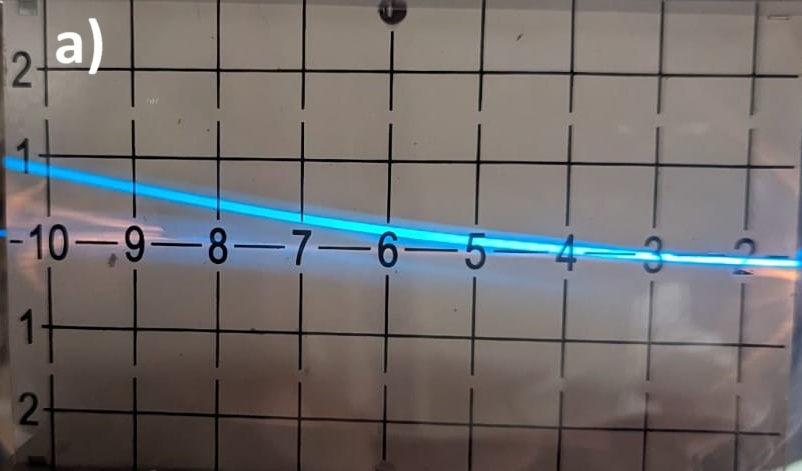
\includegraphics[width=\textwidth]{1kV.jpg}
    \end{minipage}
    \begin{minipage}{0.38\textwidth}
        \centering
        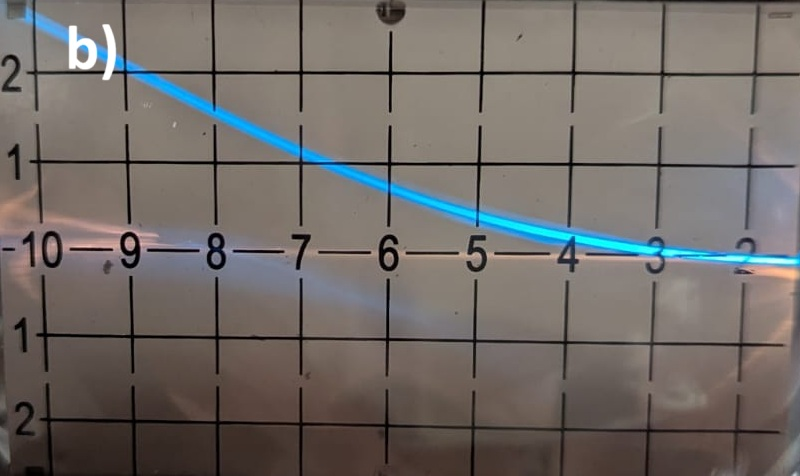
\includegraphics[width=\textwidth]{2kV.jpg}
    \end{minipage}
    \begin{minipage}{0.38\textwidth}
        \centering
        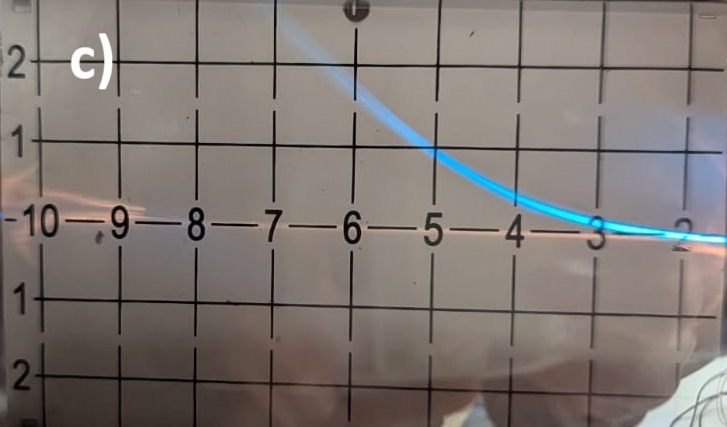
\includegraphics[width=\textwidth]{3kV.jpg}
    \end{minipage}
    \begin{minipage}{0.38\textwidth}
        \centering
        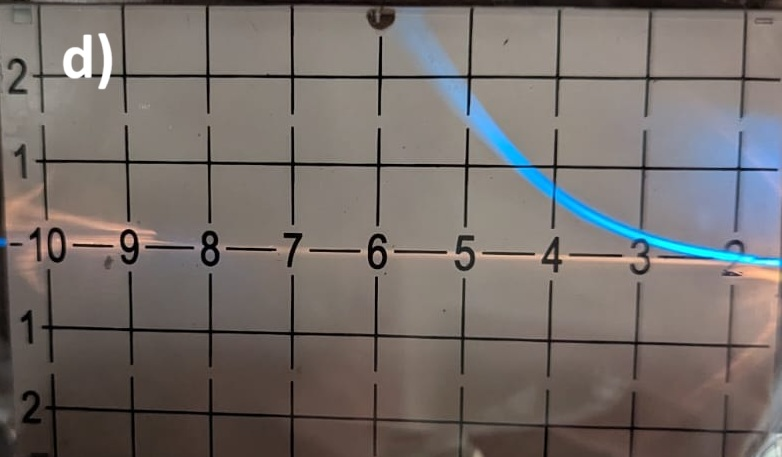
\includegraphics[width=\textwidth]{4kV.jpg}
    \end{minipage}
    \caption{Desviació del raigs en presència del camp elèctric generat per les plàques. (a) 1kV, (b) 2kV, (c) 3kV, (d) 4kV}
    \label{fig: Desv E}
\end{figure}

\subsection{Càlcul d'incerteses}\label{sec: incerteses}

\underline{Incertesa de les maangituds experimentals:} Per a magnituds experimentals obtingudes de vàries mesures hem calculat la incertesa de la següent manera: 

\begin{equation}
    \sigma_{x_i}=\sqrt{\sigma_{x_i,ins}^2+\sigma_{x_i,est}^2}
\end{equation}

Per la incertesa estadísitica s'ha agafat la desviació estàndard de les mesures i per a la incertesa instrumental hem agafat la precisió de l'insturment de mesura emprat en cada cas corresponent.

\underline{Propagació d'errors:} Per trobar les incerteses de magnituds dependents d'altres magnituds mesurables hem usat l'equació de propagació d'incerteses
\begin{equation}
    \sigma_{y}^2=\sum_{i=1}^{N}(\frac{\partial y}{\partial x_i})^2\sigma_{x_i}^2
\end{equation}
on y és la manitud dependent i ${x_i}$ les variables mesurables.

\subsection{Regressions lineals} \label{sec: Ap_Regr}

 Per fer regressions lineals que tenen en compte les incerteces individuals de cadascún dels punt hem utilitzat el mètode de mínims quadrats ponderats (weighted least squares).
 
 Donada una funció $f(x,\vec{\beta})$ a ajustar (en el nostre cas $f(x) = mx+n$):
 \begin{equation}
     f(x,\vec{\beta}) = \sum_{j=1}^m\beta_j\phi_j(x)
 \end{equation}
 
  On ${\beta_j}$ són els paràmetres a ajustar i $\phi_j$ són funcions de x (en el nostre cas $\phi_1 = x$, $\beta_1 = m$ i $\phi_2 = 1$, $\beta_2 = n$)
 
 \begin{equation}
     \hat{\beta} = (X^TWX)^{-1}X^TW\vec{y}
 \end{equation}
 \begin{equation}
     M^\beta = (X^TWX)^{-1}
 \end{equation}
 
 On $\hat{\beta}$ és l'estimador de $\beta$, $M^\beta$ la matriu de variància dels estimadors, d'on els elements de la diagonal són la desviació estàndard al quadrat dels estimadors i, per tant, l'incertesa és l'arrel quadrada dels elements de la diagonal. $W$ és la matriu (diagonal) de ponderació, $X$ és la matriu de les variables independents i $\vec{y}$ el vector de la variable dependent.
 
 \begin{equation}
     W_{ii} = \frac{1}{\sigma_i^2}
 \end{equation}
 \begin{equation}
     X_{ij} = \phi_j(x_i)
 \end{equation}

 \end{document}
